The \ThisSystem will be able to measure moisture levels and control irrigation in raised garden beds.
The purpose for \ThisSys is to maintain ideal gardening and growth conditions for fruits, vegetables, and other garden plants throughout a growing season.
The goal for \ThisSys is to automate the watering process for DIY gardeners. \ThisSys will monitor temperature, moisture levels, and additionaly environmental factors to determine when to water the plants. 
\ThisSystem is being developed by Zachary Steinberg and sponsored by University of Maryland Graduate Engineering. 
The operator and maintaner of \ThisSys will also be Zachary Steinberg. The \ThisSys will be operated outside along raised garden beds. 
\ThisSys is designed to be used by home gardeners. It is not intended for industry. \ThisSys will be controlled by a Raspberry Pi Pico W microcontroller board.

Figure~\ref{fig:SystemOverview} shows the development kit used for the \ThisSys system. 
\begin{figure}[htbp]
	\centering
		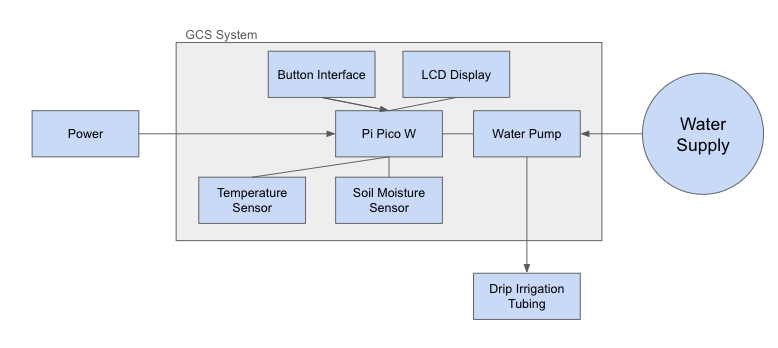
\includegraphics[width=6in]{images/SysOverview.png}
		\caption{System Overview for the \ThisSystem}
	\label{fig:SystemOverview}
\end{figure}
This diagram shows the major external interfaces that provide the capabilities of \ThisSys.
As are shown, the \ThisSys can monitor and maintain a garden system through it's environmental sesnors and control of a water pump.


% The general concept of operations (\CONOP) for this system is \TBD.





